% HW Template for CS 6150, taken from https://www.cs.cmu.edu/~ckingsf/class/02-714/hw-template.tex
%
% You don't need to use LaTeX or this template, but you must turn your homework in as
% a typeset PDF somehow.
%
% How to use:
%    1. Update your information in section "A" below
%    2. Write your answers in section "B" below. Precede answers for all 
%       parts of a question with the command "\question{n}{desc}" where n is
%       the question number and "desc" is a short, one-line description of 
%       the problem. There is no need to restate the problem.
%    3. If a question has multiple parts, precede the answer to part x with the
%       command "\part{x}".
%    4. If a problem asks you to design an algorithm, use the commands
%       \algorithm, \correctness, \runtime to precede your discussion of the 
%       description of the algorithm, its correctness, and its running time, respectively.
%    5. You can include graphics by using the command \includegraphics{FILENAME}
%
\documentclass[11pt]{article}
\usepackage{amsmath,amssymb,amsthm}
\usepackage{graphicx}
\usepackage[margin=1in]{geometry}
\usepackage{fancyhdr}
\usepackage{algorithm}
\usepackage{algpseudocode}
\usepackage{pifont}
\setlength{\parindent}{0pt}
\setlength{\parskip}{5pt plus 1pt}
\setlength{\headheight}{13.6pt}
\newcommand\question[2]{\vspace{.25in}\hrule\textbf{#1: #2}\vspace{.5em}\hrule\vspace{.10in}}
\renewcommand\part[1]{\vspace{.10in}\textbf{(#1)}}
\newcommand\algorith{\vspace{.10in}\textbf{Algorithm: }}
\newcommand\correctness{\vspace{.10in}\textbf{Correctness: }}
\newcommand\runtime{\vspace{.10in}\textbf{Running time: }}
\pagestyle{fancyplain}
\lhead{\textbf{\NAME\ (\UID)}}
\chead{\textbf{HW\HWNUM}}
\rhead{CS 6350, \today}
\begin{document}\raggedright
%Section A==============Change the values below to match your information==================
\newcommand\NAME{Jake Pitkin}  % your name
\newcommand\UID{u0891770}     % your utah UID
\newcommand\HWNUM{6}              % the homework number
%Section B==============Put your answers to the questions below here=======================

\question{1}{Probabilities}

\begin{equation}
\setlength\fboxsep{0.25cm}
\setlength\fboxrule{0.4pt}
\boxed{Independent \ Events- \ P(A \ \cap \ B) = P(A)P(B)}
\end{equation} 

\begin{equation}
\setlength\fboxsep{0.25cm}
\setlength\fboxrule{0.4pt}
\boxed{Rule \ of \ Multiplication- \ P(A \ \cap \ B) = P(A)P(B | A)}
\end{equation} 

\part{1} Given $P(A_1) = P(A_2) = P(A_1 | A_2) = \frac{1}{2}$, we want to prove that $A_1$ and $A_2$ are independent events.

Events $A_1$ and $A_2$ are independent if and only if Eq. (1) is satisfied.
$$P(A_2 \cap A_1) = P(A_2)P(A_1)$$
 We can use Eq. (2) to restate the LHS of Eq. (1) in terms of probabilities we are given.
$$P(A_2)P(A_1 | A_2) = P(A_2)P(A_1)$$
$$\frac{1}{2} * \frac{1}{2} = \frac{1}{2} * \frac{1}{2}$$

By showing Eq. (1) is satisfied, we have proven $A_1$ and $A_2$ are independent events.

\part{2} From lecture, we saw the Theorem of Total probability pertaining to mutually exclusive events $A_1, A_2, ... , A_n$ where $\sum_{i}P(A_i) = 1$. When this condition is met, we know the following is true:

$$P(B) = \sum_{i = 1}^n P(B \cap A) = \sum_{i = 1}^n P(B | A_i)P(A_i)$$

We have mutually exclusive events $A_1, A_2,$ and $A_3$ where the sum of their probabilities is 1. The condition is met, so we can use the Theorem of Total probability. All the needed probabilities to calculate $P(A_4)$ are provided in the problem.

$$P(A_4) = \sum_{i = 1}^3 P(A_4 | A_i)P(A_i)$$
$$P(A_4) = \frac{1}{3} * (\frac{1}{6} + \frac{1}{3} + \frac{1}{2})$$
\framebox[1.2\width]{$P(A_4) = \frac{1}{3}$}

\begin{equation}
\setlength\fboxsep{0.25cm}
\setlength\fboxrule{0.4pt}
\boxed{Binomial \ Distribution-  {n \choose k}p^k(1-p)^{n-k}}
\end{equation} 

\part{3} Let $X$ be a random variable representing the top of the six-sided die toss. The dice is a fair dice so we know $P(X=1) = P(X=2) = P(X=3) = P(X=4) = P(X=5) = P(X=6) = \frac{1}{6}$. There are six possible events and the total probability of exactly two heads after $n$ coin tosses is the sum of the probability of each of the six events happening. 

$$\sum_{i = 1}^6 P(X=i) * B(n = i, k = 2, p = 0.5)$$

Where $B(n, k, p)$ represents the binomial distribution from Eq. (3). This is the probability that given $n$ trials, there are exactly $k$ successes if the probability of success is $p$ where $O \leq p \leq 1$ and $k \leq n$. Let $Y$ be a random variable representing the exact number of heads after $n$ coin tosses. Note that the probability of getting exactly two heads when only tossing one coin is 0.

$$P(Y = 2) = \sum_{i = 1}^6 P(X=i) * B(n = i, k = 2, p = 0.5)$$
$$P(Y = 2) = \frac{1}{6}\sum_{i = 1}^6 B(n = i, k = 2, p = 0.5)$$
$$P(Y = 2) = \frac{1}{6}(0 + \frac{1}{4} + \frac{3}{8} + \frac{6}{16} + \frac{10}{32} + \frac{15}{64})$$
\framebox[1.2\width]{$P(Y = 2) = \frac{33}{128} = 0.2578$}

Thus this is the probability of getting exactly 2 heads after $n$ coin flips, where $n$ is the result of a fair six-sided die toss.

\begin{equation}
\setlength\fboxsep{0.25cm}
\setlength\fboxrule{0.4pt}
\boxed{Rule \ of \ Addition- \ P(A \ \cup \ B) = P(A) + P(B) - P(A)P(B|A)}
\end{equation} 

\part{4} We want to prove that if $P(A_1) = a_1$ and $P(A_2) = a_2$ then $P(A_1|A_2) \geq \frac{a_1 + a_2 -1}{a_2}$.

\textit{Proof:} we begin with Eq. (4) which is the rule for union of two events.

$$P(A_2 \cup A_1) = P(A_2) + P(A_1) - P(A_2)P(A_1 | A_2)$$

$P(A_2 \cup A_1)$ is a probability so we know it has a upper bound of 1.

$$1 \geq P(A_2 \cup A_1) = P(A_2) + P(A_1) - P(A_2)P(A_1 | A_2)$$
$$1 \geq P(A_2) + P(A_1) - P(A_2)P(A_1 | A_2)$$

Rearranging terms and multiplying both sides by -1.

$$\frac{1 - P(A_2) - P(A_1)}{P(A_2)} \geq -P(A_1 | A_2)$$
$$\frac{P(A_1) + P(A_2) - 1}{P(A_2)} \leq P(A_1 | A_2)$$

Replacing $P(A_1) = a_1$ and $P(A_2) = a_2$ on the LHS of the inequality.

$$P(A_1 | A_2) \geq \frac{a_1 + a_2 - 1}{a_2}$$

Thus arriving at the original inequality and proving it's correctness.

\part{5a} Given two independent random variables $A_1$ and $A_2$, we want to prove that $E[A_1 + A_2] = E[A_1] + E[A_2]$ is true. We will assume $A_1$ and $A_2$ are discrete for this proof. The equality also holds for continuous random variables with a slightly different proof.

Given a discrete random variable X that can take values $x_1, \ x_2, \ ..., \ x_k$, with respective probabilities $p_1, \ p_2, \ ..., \ p_k$, then the expected value of X is defined as:

\begin{equation}
\setlength\fboxsep{0.25cm}
\setlength\fboxrule{0.4pt}
\boxed{Expectation- \ E[X] = \sum_{i = 1}^k x_i * P(X = x_i)}
\end{equation} 

\textit{Proof:} Starting with the LHS of the equality we want to prove, we will use the definition of expectation to arrive at the RHS.

$$E[A_1 + A_2] = \sum_{i = 1}^k \sum_{j = 1}^k (a_{1i} + a_{2j}) * P(A_1 = a_{1i}, A_2 = a_{2j})$$

Multiply and split RHS into two sets of summations.
$$E[A_1 + A_2] = \sum_{i = 1}^k \sum_{j = 1}^k a_{1i} * P(A_1 = a_{1i}, A_2 = a_{2j})  + \sum_{i = 1}^k \sum_{j = 1}^k a_{2j} * P(A_1 = a_{1i}, A_2 = a_{2j})$$
$$E[A_1 + A_2] = \sum_{i = 1}^k a_{1i} * P(A_1 = a_{1i})  + \sum_{j = 1}^k a_{2j} * P(A_2 = a_{2j})$$

The RHS is the definition of expectation for $A_1$ summed with the expectation of $A_2$.

$$E[A_1 + A_2] = E[A_1] + E[A_2]$$

\part{5b} Given two independent random variables $A_1$ and $A_2$, we want to prove that $var[A_1 + A_2] = var[A_1] + var[A_2]$ is true.

\textit{Proof:} Variance is defined as:

\begin{equation}
\setlength\fboxsep{0.25cm}
\setlength\fboxrule{0.4pt}
\boxed{Variance - \ var[X] = E[(X - E[X])^2}
\end{equation} 

Replacing $X$ with $A_1 + A_2$ and using algebra, this can be rewritten as:

$$var[A_1 + A_2] = E[(A_1 + A_2)^2] - E[A_1 + A_2]^2$$

Expanding out the polynomials gives us:

$$var[A_1 + A_2] = E[A_1^2 + 2A_1A_2 + A_2^2] - E[A_1]^2 - 2E[A_1]E[A_2] - E[A_2]^2$$

Using the proof of linearity of expectation from part \textit{a}, we can rewrite the first expectation:

$$var[A_1 + A_2] = E[A_1^2] + 2E[A_1A_2] + E[A_2^2] - E[A_1]^2 - 2E[A_1]E[A_2] - E[A_2]^2$$ 

When the covariance of two random variables is zero, the expected value operator is multiplicative. That is, $E[XY] = E[X]E[Y]$. We know the covariance of $A_1$ and $A_2$ is 0 as they are independent of each other.

$$var[A_1 + A_2] = E[A_1^2] + 2E[A_1]E[A_2] + E[A_2^2] - E[A_1]^2 - 2E[A_1]E[A_2] - E[A_2^2]$$
$$var[A_1 + A_2] = E[A_1^2] - E[A_1]^2 + E[A_2^2] - E[A_2^2]$$

Arriving at the definition of variance after it is expanded out with algebra:

$$var[A_1 + A_2] = var[A_1] + var[A_2]$$

\question{2}{Na\"{i}ve Bayes}

\part{1a} Given infinite data drawn from this distribution, the learned probabilities $\hat P$ will be identical to the true probabilities $P$. This is a result of the law of large numbers.

$$\hat P(y = -1) = 0.1 \ and \ \hat P(y = 1) = 0.9$$
$$\hat P(x_1 = -1 | y = -1) = 0.8 \ and \  \hat P(x_1 = 1 | y = -1) = 0.2$$
$$\hat P(x_1 = -1 | y = 1) = 0.1  \ and \ \hat P(x_1 = 1 | y = 1) = 0.9$$ 

\part{1b} Using the conditional independence assumption the naive Bayes model makes, we can calculate the generative distribution of the data using $\hat P(x_1, y) = \hat P(y) \hat P(x_1 | y)$. A prediction $y^\prime$ is determined by taking the maximum of the $\hat P(x_1, y)$ for a given value of $x_1$.

\begin{table}[H]
\centering
{\renewcommand{\arraystretch}{1.2}%
\begin{tabular}{| c | c | c | c |}
\hline
$x_1$ & $\hat P(x_1, y = -1)$ & $\hat P(x_1, y = 1)$ & \textbf{Prediction:} $y^\prime = argmax_y \hat P(x_1, y)$\\
\hline
-1 & (0.1)(0.8) = \textbf{0.08} & (0.9)(0.1) = \textbf{0.09} & 1\\ \hline
1 & (0.1)(0.2) = \textbf{0.02} & (0.9)(0.9) = \textbf{0.81} & 1\\ \hline
\end{tabular}}
\end{table}

\part{1c} To determine the error of the classifier, we calculate the probability of $P(y^\prime \neq y)$ being true. To calculate this we can use the fact that $P(y^\prime \neq y) = P(y^\prime \neq y, x_1 = -1) + P(y^\prime \neq y, x_1 = 1)$, using the values from the table in part b.

$$P(y^\prime \neq y) = P(y = -1 | x_1 = -1) + P(y = -1 | x_1 = 1)$$
$$P(y^\prime \neq y) = (0.1)(0.8) + (0.1)(0.2) = 0.1$$

If we trained a classifier on the given data, it would have an error rate of $\mathbf{0.1}$.

\part{2a} The two features $x_1$ and $x_2$ are not conditionally independent given $y$.

\textit{Proof:} From lecture we saw the definition of conditional independence of three random variables. The random variables are independent if and only if the equality is satisfied.

$$P(X, Y|Z) = P(X|Z)P(Y|Z)$$
$$P(x_1, x_2|y) = P(x_1|y)P(x_2|y)$$

As $x_1$ and $x_2$ are identical, $P(x_1, x_2 | y)$ is the same as $P(x_1 |y)$ as $x_1$ and $x_2$ always happen or don't happen together. Replacing $P(x_1, x_2 |y)$ with $P(x_1 | y)$ in the conditional independence formula.

$$P(x_1 | y) = P(x_1 | y)P(x_2 | y)$$

We know our given probabilities are non-zero, thus the above equality does not hold. Proving $x_1$ and $x_2$ are not conditionally independent.

\part{2b} As in part 1, using the conditional independence assumption the naive Bayes model makes, we can use $\hat P(x_1 | y)$, $\hat P(x_2 | y)$, and $\hat P(y)$ to calculate the generative distribution of the data.

$$\hat P(x_1, x_2, y) = \hat P(y) \hat P(x_1 | y) \hat P(x_2 | y)$$

\begin{table}[H]
\centering
{\renewcommand{\arraystretch}{1.2}%
\begin{tabular}{| c | c | c | c | c |}
\hline
$x_1$ & $x_2$ & $\hat P(x_1, x_2, y = -1)$ & $\hat P(x_1, x_2, y = 1)$ & \textbf{Prediction:} $y^\prime = argmax_y \hat P(x_1, x_2, y)$\\
\hline
-1 & -1 & (0.1)(0.8)(0.8) = \textbf{0.064} & (0.9)(0.1)(0.1) = \textbf{0.009} & -1\\ \hline
-1 & 1 & (0.1)(0.8)(0.2) = \textbf{0.016} & (0.9)(0.1)(0.9) = \textbf{0.081} & 1\\ \hline
1 & -1 & (0.1)(0.2)(0.8) = \textbf{0.016} & (0.9)(0.9)(0.1) = \textbf{0.081} & 1\\ \hline
1 & 1 & (0.1)(0.2)(0.2) = \textbf{0.004} & (0.9)(0.9)(0.9) = \textbf{0.729} & 1\\ \hline
\end{tabular}}
\end{table}

\part{2c} To determine the error of the classifier, we calculate the probability of $P(y^\prime \neq y)$ being true. To calculate this we can use the fact that $P(y^\prime \neq y) = P(y^\prime \neq y, x_1 = -1, x_2 = -1) + P(y^\prime \neq y, x_1 = -1, x_2 = 1) + P(y^\prime \neq y, x_1 = 1, x_2 = -1) + P(y^\prime \neq y, x_1 = 1, x_2 = 1)$, using the values from the table in part b.

$$P(y^\prime \neq y) = 0.009 + 0.016 + 0.016 + 0.004 = 0.045$$

If we trained a classifier on the given data, it would have an error rate of \textbf{0.045}.

\part{2d} Both na\"ive Bayes (generative) and logistic regression (discriminative) compute the same posterior distribution over the outputs. But, discriminative models don't characterize the distribution of the inputs where a generative model does.

So no, I don't expected the duplication of a variable to have the same results in logistic regression as we saw in na\"ive Bayes.

\question{3}{Na\"{i}ve Bayes and Linear Classifiers} Our classifier will predict a label of 1 if the following is true:

\begin{equation}
\frac{Pr(x|y = 1)Pr(y=1)}{Pr(x|y = 0)Pr(y = 0)} \geq 1
\end{equation}

We saw in class that the na\"ive Bayes classifier makes the assumption that all features $x_j$ are independent of each other. This allows for a simplified calculation for a conditional probability:

\begin{equation}
Pr(\mathbf{x}|y) = \prod_{j=0}^d Pr(x_j|y)
\end{equation}

This allows us to rewrite the condition for predicting a label of 1 from Eq. (7):

\begin{equation}
\frac{Pr(y=1)}{Pr(y=0)} * \prod_{i = 0}^d \frac{Pr(x_j | y = 1)}{Pr(x_j | y = 0)} \geq 1
\end{equation}

Suppose each $Pr(x_j|y)$ is defined using a Gaussian/Normal probability density function, one for each value of $y$ and $j$. Each Gaussian distribution has mean $\mu_{j,y}$ and variance $\sigma^2$. We can rewrite the $Pr(x_j|y)$ in Eq. (9) in terms of their Gaussian functions. Additionally we will replace $Pr(y = 1)$ with $p$ and $Pr(y = 0)$ with $p - 1$.

\begin{equation}
\frac{p}{p-1} * \prod_{i = 0}^d \frac{\frac{1}{\sqrt{2\sigma^2\pi}}e^{\frac{-(x_j-\mu_{j,1})^2}{2\sigma^2}}}{\frac{1}{\sqrt{2\sigma^2\pi}}e^{\frac{-(x_j-\mu_{j,0})^2}{2\sigma^2}}} \geq 1
\end{equation}

Our goal is to get Eq. (10) in the form of a familiar linear model. First, we group all the constant terms that don't rely on a $x_j$ term.

\begin{equation}
\Bigg( \frac{p}{p-1}\prod_{i = 0}^d \frac{\frac{1}{\sqrt{2\sigma^2\pi}}}{\frac{1}{\sqrt{2\sigma^2\pi}}} \Bigg) * \prod_{i = 0}^d \frac{e^{\frac{-(x_j-\mu_{j,1})^2}{2\sigma^2}}}{e^{\frac{-(x_j-\mu_{j,0})^2}{2\sigma^2}}} \geq 1
\end{equation}

Apply the log rule $e^{-x}/e^{-y} = e^{y-x}$:

\begin{equation}
\Bigg( \frac{p}{p-1}\prod_{i = 0}^d \frac{\frac{1}{\sqrt{2\sigma^2\pi}}}{\frac{1}{\sqrt{2\sigma^2\pi}}} \Bigg) * \prod_{i = 0}^d e^{\frac{(x_j-\mu_{j,0})^2}{2\sigma^2} - \frac{(x_j-\mu_{j,1})^2}{2\sigma^2}} \geq 1
\end{equation}

Then we will take the natural log of both sides of the equation:

\begin{equation}
log \Bigg( \frac{p}{p-1}\prod_{i = 0}^d \frac{\frac{1}{\sqrt{2\sigma^2\pi}}}{\frac{1}{\sqrt{2\sigma^2\pi}}} \Bigg) * \sum_{i = 0}^d \frac{(x_j-\mu_{j,0})^2}{2\sigma^2} - \frac{(x_j-\mu_{j,1})^2}{2\sigma^2} \geq 0
\end{equation}

Expanding the squares, canceling like terms and factoring $x_j$ out:

\begin{equation}
log \Bigg( \frac{p}{p-1}\prod_{i = 0}^d \frac{\frac{1}{\sqrt{2\sigma^2\pi}}}{\frac{1}{\sqrt{2\sigma^2\pi}}} \Bigg) * \sum_{i = 0}^d x_j * \frac{2\mu_{j,1} - 2\mu_{j,0}}{2\sigma^2} \geq 0
\end{equation}

Let us denote the grouped constant terms outside the summation by $b$ and let us denote $\frac{2\mu_{j,1} - 2\mu_{j,0}}{2\sigma^2}$ by $w_j$:

\begin{equation}
b + \sum_{i = 0}^d x_jw_j \geq 0
\end{equation}

Recall if the original Eq. (7) was true we should predict a label of 1. Thus, we have shown Eq. (7) is a linear classifier.

\question{4}{Experiment}

\part{1} 
$$g(W) = log(1 + exp(-y_i\mathbf{w^Tx_i}))$$

We want to calculate $\frac{dg}{dw}$, or the derivative of the function $g$ in terms of $\mathbf{w}$. We can use the chain rule where $a = 1 + exp(-y_i\mathbf{w^Tx_i})$ and $b = -y_i\mathbf{w^Tx_i}$.

$$\frac{d}{da} \ log(a) = \frac{1}{a}$$
$$\frac{d}{db} \ 1 + exp(b)= exp(b)$$
$$\frac{d}{dw} \ -y_i\mathbf{w^Tx_i} = -y_i\mathbf{x_i}$$
Computing the derivative of the composition of the three functions using the chain rule:
$$\frac{dg}{dw} = \frac{dg}{da} * \frac{da}{db} * \frac{db}{dw}$$
$$\frac{dg}{dw} = \frac{1}{a} * e^b * -y_i\mathbf{x_i}$$
$$\frac{dg}{dw} = \frac{1}{1 + exp(-y_i\mathbf{w^Tx_i})} * exp(-y_i\mathbf{w^Tx_i}) * -y_i\mathbf{x_i}$$

\begin{equation}
\setlength\fboxsep{0.25cm}
\setlength\fboxrule{0.4pt}
\boxed{\frac{dg}{dw} = \frac{-y_i\mathbf{x_i}}{1 + exp(y_i\mathbf{w^Tx_i})}}
\end{equation} 

\part{2} When the entire dataset is composed of a single example, the objective is expressed as:

\begin{equation}
\setlength\fboxsep{0.25cm}
\setlength\fboxrule{0.4pt}
\boxed{objective:\ J(w) = log(1 + exp(-y_i\mathbf{w^tx_i})) + \frac{1}{\sigma^2}\mathbf{w^Tw}}
\end{equation}

This is equivalent to the original optimization problem as finding the min of a summation is redundant when taking only one example.

The gradient of this objective can be found using the derivative found in part $1$ plus the derivative of $\frac{1}{\sigma^2}\mathbf{w^Tw}$. We use the fact that $w^Tw = w^2$.

\begin{equation}
\setlength\fboxsep{0.25cm}
\setlength\fboxrule{0.4pt}
\boxed{\nabla J(w) = \frac{-y_i\mathbf{x_i}}{1 + exp(y_i\mathbf{w^Tx_i})} + \frac{2\mathbf{w}}{\sigma^2}}
\end{equation}

\part{3} Using the objective $J(w)$ (Eq. 8) and the gradient $\nabla J(w)$ (Eq. 9) from the previous part, we can write pseudo code for a stochastic gradient descent algorithm. Recall in stochastic gradient descent we treat a random example as the full dataset.
\vspace{2mm} \break
{\Large \textbf{Stochastic gradient descent for logistic regression classifier}} \vspace{2mm} \break
{\large Given a training set S = \{($\mathbf{x_i}, y_i$)\}, $\mathbf{x} \in \Re^n$, $y \in \{-1, 1\}$:} \vspace{2mm} \break
{\large 1. \hspace{5mm} Initialize $\mathbf{w}^0 = 0 \in \Re^n$} \vspace{2mm} \break
{\large 2. \hspace{5mm} For epoch = 1 ... T:} \vspace{2mm} \break
{\large \hspace*{20mm} 1. For each shuffled training example ($\mathbf{x_i}$, $y_i) \in S$:} \vspace{2mm} \break
{\large \hspace*{20mm} 2. Take the derivative of $J(w)$, where the current example represents the entire}
{\large \hspace*{25mm} dataset, at the current $\mathbf{w^{t-1}}$ to be $\nabla J^t(\mathbf{w^{t-1})}$} \vspace{2mm} \break
{\large \hspace*{20mm} 3. Update: $\mathbf{w^t} = \mathbf{w^{t-1}} - \gamma \nabla J^t(\mathbf{w^{t-1}})$} \vspace{2mm} \break
{\large 3. Training is done, return the weight vector $\mathbf{w}$}

\part{4} \textit{Cross validation:} I performed cross validation to determine the best learning rate $\gamma$ and $\sigma^2$ for the Adult data set. For each combination of $\gamma \in \{1, \ 0.5, \ 0.1, \ 0.05, \ 0.01, \ 0.001\}$ and $\sigma \in \{10, \ 20, \ 25, \ 50, \ 100, \ 1,000\}$ 6-cross validation was performed. Below is a table of interesting results including the best and worst performing hyper-parameters.

\begin{table}[H]
\centering
{\renewcommand{\arraystretch}{1.2}%
\begin{tabular}{| c | c | c | c |}
\hline
$\gamma$ & $\sigma$ & Epoch & Accuracy\\
\hline
1 & 25 & 1 & 0.594\\ \hline
0.01 & 10 & 1 & 0.835\\ \hline
0.01 & 50 & 1 & 0.845\\ \hline
0.01 & 1,000 & 1 & 0.844\\ \hline
0.0001 & 25 & 1 & 0.756\\ \hline
\end{tabular}}
\caption{Interesting results from 6-fold cross validation.}
\end{table}

I found $\sigma$ to have little to no weight on the accuracy of the classifier. This can be seen in the middle three results from the table, regardless of the $\sigma$ chosen the accuracy remains the same. I found the choice of $\gamma$ to be the determiner in the accuracy of the classifier. A large $\gamma$ such as 1 or a smaller $\gamma$ such as 0.0001 caused poor results. It should be noted that 0.76 is a baseline for this dataset as predicting all -1 gives this accuracy. \textbf{I found the best $\gamma$ to be 0.01 when paired with a $\sigma$ of 50}.

\textit{Experiment:} With the found best $\gamma$ of 0.01 and $\sigma$ of 50, I trained stochastic gradient descent algorithm on the Adult training data. Once trained, I evaluated it's performance on the Adult training and Adult test data.

\begin{table}[H]
\centering
{\renewcommand{\arraystretch}{1.2}%
\begin{tabular}{| c | c | c | c | c |}
\hline
Data Set & $\gamma$ & $\sigma$ & Epoch & Accuracy\\
\hline
Adult training & 0.01 & 50 & 200 & 0.85\\ \hline
Adult testing & 0.01 & 50 & 200 & 0.847\\ \hline
\end{tabular}}
\caption{Classification accuracy on the Adult training and test set.}
\end{table}

Below is a plot of the objective after each epoch of SGD. For this plot, SGD was ran on the Adult training set with a $\gamma$ of 0.01, a $\sigma$ of 50, and a epoch of 200.

\begin{figure}[H]
  \centerline{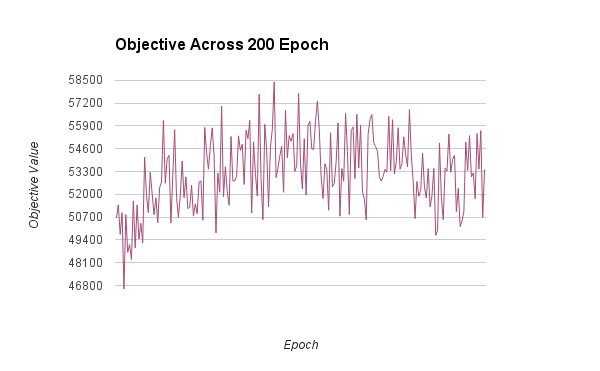
\includegraphics[width=1\linewidth]{objective.png}}
\end{figure}

\end{document}
